\chapter{Hauptteil}
\label{cha:Hauptteil}

\section{Zugrundeliegende Rechnungen}
\label{sec:zugrundeliegende}

Die ersten Berechnungsansätze für Sprinklerauslösezeiten mithilfe des RTI wurden bereits 1980 durch Heskestad und Smith aufgestellt.\footnote{G. Heskestad and H. F. Smith, \emph{Plunge Test for
Determination of Sprinkler Sensitivity}, Factory Mutual Research Corporation, Norwood, MA, December, 1980. Zitiert nach \cite{Heskestad1988}.}
Die aktuelle VDI-Richtlinie 6019-1 aus dem Jahr 2006 beschreibt den Rechenweg zur Ermittlung der Sprinklerauslösezeiten \cite{VDI6019B1}.
Die Richtlinie bezieht sich für die Vorhersage von Rauchgastemperatur und -geschwindigkeit auf das \emph{SFPE Handbook of Fire Protection Engineerung, $2^{nd}$Edition} aus dem Jahr 1995, welches sich wiederum auf eine wissenschaftliche Veröffentlichung von Heskestad und Delichatsios aus dem Jahr 1979 \cite{Heskestad1979} bezieht. Den beiden Wissenschaftlern fiel im Nachhinein allerdings auf, dass sie einen falschen Heizwert für Holz verwendet hatten und somit die aufgestellten Formeln fehlerhaft waren. Dieser Fehler wurde zehn Jahre später in einer weiteren Veröffentlichung korrigiert \cite{Heskestad1989}. Die Korrektur wurde dann im Jahre 2002 vom SFPE Handbook Third Edition \cite{SFPE3rd} aufgegriffen. 
Die SFPE Handbücher (mittlerweile in der fünften Edition) der Society of Fire Protection Engineers gelten als unumgängliche Literatur im Bereich des Brandschutzes. 

Somit ist klar, dass die den Tabellen zugrundeliegenden Formeln in der VDI-Richtlinie nicht mehr den korrekten wissenschaftlichen Erkenntnisstand widerspiegeln. Es hat sich im Laufe der Arbeiten zur Überarbeitung der Richtlinie herausgestellt, dass die Sprinklerauslösezeiten mit den veralteten Formeln unter manchen Parametern bis zu einem Drittel größer waren als mit den neuen Formeln. Dadurch, dass die Auslösezeiten überschätzt wurden, bestand zu keinem Zeitpunkt eine Gefahr für Menschen durch falsch dimensionierte Anlagentechnik oder Brandschutzkonzepte.

Ein weiterer Punkt, den es zu beachten gilt, ist die eigentliche Formel für die Sprinklerauslösezeit. Die Autoren der VDI-Richtlinie beziehen sich in Gl. \ref{eq:VDISprinkleraktivierung} auf eine wissenschaftliche Veröffentlichung aus dem Jahr 1999 \cite{Davis1999}, welche sich wiederum auf ein Paper von Heskestad bezieht \cite{Heskestad1988}. Hier wird im Gegensatz zum SFPE Handbuch 3rd Ed. noch mit dem C-Faktor gerechnet.
Das Handbuch besagt ab der dritten Edition, dass die Glasfässchen in den Sprinklerköpfen meist thermisch isoliert vom Rest des Sprinklerkopfes zu betrachten sind und somit der Wärmeleitungsanteil im Vergleich zum Konvektionsanteil vernachlässigbar sei \cite[Kap. 4, S. 5]{SFPE3rd}. Dies steht im Widerspruch zu einer Arbeit von Kokkala, der dem Wärmeverlust durch Wärmeleitung auf bis zu 10~\% ansetzt.\footnote{M. Kokkala, \emph{Thermal Properties of Heat Detectors
and Sprinklers}, Nordtest Brand Symposium, Boras,
Sweden (1986). Zitiert nach \cite[Kap. 4, S. 6]{SFPE3rd}.} 
Somit ist noch unklar, inwiefern der C-Faktor zur Simulation von Brandszenarien beiträgt. Dies gilt es zusätzlich in dieser Arbeit zu untersuchen. In den nachfolgenden Sektionen werden die zugrundeliegenden Formeln der VDI 6019 Blatt 1 und des SFPE Handbuches 3rd Ed. betrachtet. Zur besseren Verständlichkeit wurden Formeln zusammengefasst und Symbole und Indizes angeglichen.






\subsection{Berechnung nach VDI 6019-1}
\label{BerechnungenausVDI}

Mithilfe der nachfolgenden Formeln kann die Sprinklerelementtemperatur $T_e$ zum Zeitpunkt $t$ nach der VDI-Richtlinie bestimmt werden: 

\begin{align}
    \frac{\mathrm{d} T_{e}}{\mathrm{d} t}=&\frac{\sqrt{u}}{\mathrm{RTI}}\cdot \left [ T_g-T_{e}-\frac{C}{\mathrm{\sqrt{u}}}\cdot \left(T_{e}-T_{\infty}\right) \right ] \label{eq:VDISprinkleraktivierung}\\[20pt]
    \intertext{durch das Lösen der DGL folgt nach Heskestad \cite{Heskestad1988}:} \nonumber\\
    \Delta T_e &= T_e(t)-T_0=\frac{\Delta T_g}{1+C/\sqrt{u}}\left [ 1-\text{exp} \left( -\; \frac{t \sqrt{u}(1+C/\sqrt{u})}{\text{RTI}} \right ) \right ] \label{eq:3.2}\\[20pt]
    \intertext{die Rauchgastemperatur $T_g$ und die Rauchgasgeschwindigkeit $u$ am Sprinklerkopf werden mit folgenden Formeln berechnet:} \nonumber\\
    \Delta T_g&= T_g(t)-T_g(t_0)=\Delta T_{2}^{*} \cdot\left[K^{2 / 5}\left(T_{\infty} / g\right) \alpha^{2 / 5} H^{\,-3 / 5}\right] \label{eq:3.4}\\[20pt]
    u&=u^*_2\cdot \left ( K^{1/5}\alpha^{1/5}H^{1/5} \right ) \label{eq:3.3}\\[20pt]
     \intertext{mit:} \nonumber\\
     \Delta T_{2}^{*}&=
        \begin{dcases}
        {\hspace{68pt}0} &
        {t_2^* \leq t_{f}^{*}} \\[20pt]
        {\left(\frac{t_{2}^{*}-t_{1}^{*}}{0{,}188+0{,}313 \cdot r / H }\right )^{4/3}}&
{t_2^*>t_{f}^{*}}
\end{dcases} \label{eq:3.5}\\[20pt]
   t^*_2&=\frac{t_0}{K^{-1/5}\alpha^{-1/5}H^{\,4/5}} \label{eq:3.6}\\[20pt]
   t^*_f&=0{,}954(1+r/H)\label{eq:3.7}\\[20pt]
   u^*_2&=0{,}59(r/H)^{-0{,}63}\cdot \sqrt{\Delta T^*_2} \label{eq:3.8}\\[20pt]
   \intertext{Nachfolgendende Gleichung beschreibt die Stoffwertkonstante. Die Stoffwerte für die Konstante werden in der VDI-Richtlinie nicht vorgegeben.} \nonumber\\
   K&=\frac{g}{c_p\cdot T_\infty \cdot \rho_\infty}\label{eq:3.9}
\end{align}

\SuperPar

hierbei ist:
\begin{align*}
  T_e &\qquad \text{Sprinklerelementtemperatur in K} \\[3pt]
  T_g &\qquad \text{Rauchgastemperatur am Sprinklerkopf} \\[3pt]
  u &\qquad \text{Rauchgasgeschwindigkeit am Sprinklerkopf} \\[3pt]
  \text{C} &\qquad \text{Wärmeleitfaktor in (m/s)$^{0,5}$} \\[3pt]
  \text{RTI} &\qquad \text{Response Time Index in (m$\cdot$s)$^{0,5}$} \\[3pt]
  \Delta T^*_2 &\qquad \text{dimensionslose Rauchgastemperatur} \\[3pt]
  u^*_2 &\qquad \text{dimensionslose Rauchgasgeschwindigkeit} \\[3pt]
  t^*_f &\qquad \text{dimensionslose Vorlaufzeit} \\[3pt]
  t^*_2 &\qquad \text{dimensionslose Zeit} \\[3pt]
  K &\qquad \text{Stoffwertkonstante} \\[3pt]
  \alpha &\qquad \text{Brandintensitätskoeffizient in kW/s²} \\[4pt]
  r &\qquad \text{Vertikaler Abstand zwischen Brandherd und Auslöseelement in m} \\[4pt]
  H &\qquad \text{Abstand zwischen Brandherd und Decke in m} \\[4pt]
  \rho_\infty &\qquad \text{Dichte der Luft in kg/m³}  \\[4pt]
  c_p &\qquad \text{spezifische Wärmekapazität in kJ/(kg}\cdot\text{K)} \\[4pt]
  g & \qquad \text{Erdbeschleunigung in m/s²}
\end{align*}
 Aus den Formeln ist kein Hinweis auf den konvektiven Anteil des Brandintensitätskoeffizienten ersichtlich, obwohl er in Kap. 3.7 der Richtlinie thematisiert wird.

\subsection{Berechnungen nach SFPE Handbook 3rd Ed.}
\label{sec:Berechnungennachsfpe}

Die nachfolgenden Formeln des SFPE Handbuches verwenden größtenteils die gleichen Parameter und Hilfsvariablen wie die VDI-Richtlinie \bzw die Heskestad Paper. Allerdings wird hier mit dem konvektiven Brandintensitätskoeffizienten $\alpha_c$ gerechnetm, der mit Gl. \ref{eq:3.15} bestimmt werden kann. 

\begin{align}
    \Delta T_e&=\frac{\Delta T_g}{\Delta T^*_2}\,\Delta T^*_2 \left [ 1-\frac{(1-e^{-\gamma})}{\gamma}\right ]\label{eq:3.10} \\[20pt]
    \intertext{mit:} \nonumber\\
    \frac{\Delta T_g}{\Delta T^*_2}&=K^{2/5}(T_\infty/g)\,\alpha^{2/5}_c\,H^{-3/5} \label{eq:3.11}\\[20pt]
    \Delta T^*_2&=\left [ \frac{\left (t^*_2-t^*_{2f} \right )}{\left (0{,}126+0{,}210\cdot r/h \right )}    \right ] \label{eq:3.12}\\[20pt]
    \gamma &= \frac{3}{4}\sqrt{\frac{u}{u^*_2}}\sqrt{\frac{u^*_2}{(\Delta T^*_2)^{1/2}}}\left ( \frac{\Delta T^*_2}{RTI} \right ) \left ( \frac{t}{t^*_2} \right ) \left ( 0{,}126+0{,}210 \frac{r}{H} \right )\label{eq:3.13} \\[20pt]
    \alpha_c&=X\cdot\alpha \label{eq:3.15}\\[20pt]
    \frac{u}{u^*_2}&=K^{2/5}\alpha^{2/5}H^{-3/5}\label{eq:3.16}\\[20pt]
    t^*_2&=\frac{t}{K^{-1/5}\alpha^{-1/5}_c H^{\,4/5}}\label{eq:3.17}\\[20pt]
    t^*_{2f}&=0{,}813\left (1+\frac{r}{H} \right )\label{eq:3.18}\\[20pt]
    \frac{u^*_2}{(\Delta T^*_2)^{1/2}}&=0{,}59 \left ( \frac{r}{H}\right )^{-0{,}63}\label{eq:3.19}  
    \intertext{Die Stoffwerte des Rauchgases für die Stoffwertkonstante sind nach \cite[Kap.4, S.15]{SFPE3rd} wie folgt vorgegeben: $c_p=1{,}04$ kJ/(kg$\cdot$K), $\rho_\infty=1{,}1$ kg/m³ und $g=9{,}81$ m/s².} \nonumber\\
    K&=\frac{g}{c_p \cdot T_\infty \cdot \rho_\infty}\label{eq:3.14} \\[20pt]
\end{align}

\SuperPar hierbei ist:
\begin{align*}
    \gamma &\qquad \text{Argument für die Exponentialfunktion} \\[3pt]
    X &\qquad \text{Konvektionsanteil} \\[3pt]
    \alpha_c &\qquad \text{konvektiver Brandintensitätskoeffizient}
\end{align*}





\section{FDS Hintergrund}
\label{sec:FDSHintergrund}

\subsection{Einführung FDS und Smokeview}
\label{sec:EinfuehrungFDS}

FDS (Fire Dynamics Simulator) \cite{FDSWebsite} ist eine der bekanntesten CFD-Software (Computational Fluid Dynamics) zur Modellierung von Szenarien auf dem Gebiet des Brandschutzes. Entwickelt durch das amerikanische National Institute of Standards and Technology (NIST), bietet es eine Reihe von Möglichkeiten zur Simulation unterschiedlichster Brand\-szenarien. 
Um turbulente Strömungen zu modellieren, benutzt FDS die Methode der Large Eddy Simulation (LES). Dies ist ein Verfahren, bei der numerische Berechnungen angestellt werden und mittels eines Tiefpassfilters Navier-Stokes-Gleichungen örtlich und zeitlich gefiltert werden. Große Wirbelstrukturen können somit direkt berechnet werden, während kleine Strukturen über ein Feinstrukturmodell abgebildet werden. Die Aussagekraft und Rechenzeit liegt damit unter dem Verfahren der direkten numerischen Simulation, aber über der Lösung der RANS-Gleichungen (Reynolds-Averaged-Navier-Stokes) \cite{WikiLES}.
Simulationsparameter werden in eine vom Nutzer erstellte Textdatei eingegeben. Diese wird dann in der Konsole aufgerufen und von FDS eingelesen und kompiliert. Anschließend erfolgt die visuelle Darstellung der Ergebnisse mithilfe der dazugehörigen Smokeview Software. Diese kann Feuer, Rauch und Partikel aus der FDS Berechnung darstellen. Außerdem ist es möglich, sich mithilfe der richtigen Voreinstellungen in der FDS Input-Datei 2D Schnitte und 3D Plots grafisch ausgeben zu lassen. Daten wie \zB die Wärmefreisetzungsrate und Sprinklerkopftemperatur werden im Dateiformat CSV (Comma-separated values) gespeichert.

Für die Simulationen mit FDS wird mit einem Computercluster gerechnet. Dieser besitzt über zwei Prozessoren verteilt insgesamt 28 Kerne. Jeder Kern besitzt zwei Threads.\footnote{Abläufe eines Computerprogramms, die in Multitaskingumgebungen unabhängig von und zeitgleich mit anderen ausgeführt werden können.} FDS wird in der Version 6.7.3 und Smokeview in der Version 6.7.10 verwendet.

\subsection{FDS Formel für Sprinkleraktivierung}
\label{sec:technHintergrund}

In FDS wird die Sprinklerauslösetemperatur mit einer umgestellten Version der ursprünglichen Formel nach Heskestad \cite{Heskestad1988} berechnet (siehe Gl. \ref{eq:FDSSprinkler}) und somit ist auch der C-Faktor inkludiert. FDS setzt diesen bei fehlender Nutzereingabe standardmäßig auf 0,7~(m/s)$^{0,5}$. $T_m$ stellt hier die Temperatur des eigentlichen Sprinklerkopfes und der Sprinklerkopffassung dar, an die das Glasfässchen seine Wärme abgibt. Die Software nimmt an, dass $T_m$ der Umgebungstemperatur entspricht \cite{FDSTech}, obwohl sich der Sprinklerkopf auch der Gas\-temperatur anpasst.

Der rechts äußerste Term ist für die Abkühlung des Sprinklerkopfes durch das freigesetzte Löschwasser hinzugefügt worden. Dieser spielt für diese Arbeit keine Rolle, da nur die Aktivierung eines einzigen Sprinklerkopfes betrachtet wird. Wenn mehrere Sprinklerköpfe in einer Simulation untersucht werden, kommt es zu einer gegenseitigen Beeinflussung der Sprinklerköpfe, da die Brandquelle und der Rauch durch die Wasserpartikel abgekühlt werden. 


\begin{equation}
\label{eq:FDSSprinkler}
\frac{\mathrm{d} T_{e}}{\mathrm{d} t}=\frac{\sqrt{|\mathbf{u}|}}{\mathrm{RTI}}\left(T_{g}-T_{e}\right)-\frac{C}{\mathrm{RTI}}\left(T_{e}-T_{\infty}\right)-\frac{C_{2}}{\mathrm{RTI}} \beta|\mathbf{u}|
\end{equation}




\subsection{FDS Validierung}
\label{sec:FDSVal}

Der Validierungsprozess soll determinieren, wie gut das zugrundeliegende mathematische Modell das zu betrachtende physikalische Phänomen vorhersagt \cite{FDSVal}. Hierbei wird untersucht, ob Ergebnisse aus realen Versuchen mit den Simulationsergebnissen übereinstimmen \bzw wie viel sie voneinander abweichen. 

FDS liegt ein Validierungsführer bei, welcher auf verschiedene Experimente und Simulationen eingeht und diese miteinander vergleicht. Für die Sprinkleraktivierung wurden bereits einige Versuche und Simulationen angestellt, die die Validität von FDS in Bezug auf das Sprinklermodell bestätigen. Abb. \ref{fig:SprinklerVal} stellt alle Ergebnisse aus den Realversuchen (\emph{X-Achse}) denen aus den FDS Simulationen (\emph{Y-Achse}) gegenüber. Der Faktor der Verzerrung der Simulationsfunktion liegt bei 1,02 und die relative Standardabweichung beträgt $\pm 16\; \%$. Man erkennt eine gute Übereinstimmung der Ergebnisse zwischen den Realversuchen und den FDS Simulationen.
\begin{figure}
    \centering
    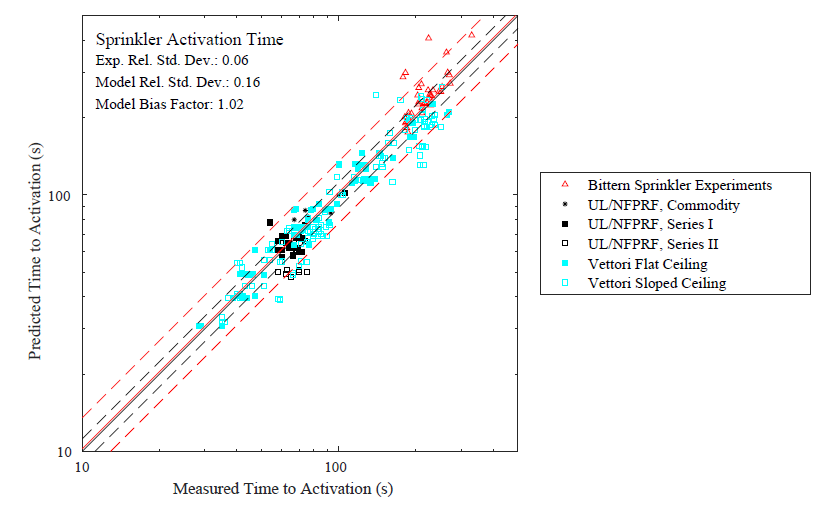
\includegraphics[width=.9\textwidth]{images/SprinklerValidation.PNG}
    \caption{Vergleich zwischen gemessenen und simulierten Sprinkleraktivierungszeiten  \cite{FDSVal}.}
    \label{fig:SprinklerVal}
\end{figure}



\section{FDS Modell}
\label{sec:FDSModell}
 
\subsection{Mesheinteilung}
\label{sec:endgueltigeMesheinteilung}

Simulationen in FDS müssen innerhalb vordefinierter Raumgrenzen ablaufen. Diese Raumgrenzen werden von mindestens einem Mesh gefüllt. Mesh bestehen aus vielen kleineren kubischen Volumenkörpern, den sogenannten Zellen. Diese Zellen füllen ein Gitterraster (auch "`Grid"' genannt) aus, welches das Mesh in die verschiedenen Zellen aufteilt. Die Anzahl dieser Zellen pro Mesh beruht auf der gewünschten Auflösung der Simulation. Generell kann angenommen werden, dass je höher die Auflösung der Simulation, desto höher die Genauigkeit der Ergebnisse. Mit einer erhöhten Zellenanzahl steigt allerdings auch die Rechenzeit für die Simulation. Diese kann bei Millionen von Zellen zur Folge haben, dass auch mit leistungsfähigen Computern die Rechenzeit mehrere Tage oder Wochen beträgt. 
Somit muss ein Kompromiss zwischen der Rechengenauigkeit und der Rechenzeit gefunden werden. Generell sollte zuerst mit einer niedrigen Auslösung gerechnet werden, um diese dann schrittweise zu erhöhen bis keine signifikanten Unterschiede bei den Ergebnissen mehr festgestellt werden. Dies wird eine Mesh Sensitivity Study (siehe Kap. \ref{sec:MeshSS}) genannt. Um die große Leistung des Clusters vollständig ausnutzen zu können, wird der Raum in mehrere Mesh aufgeteilt. 
Hier sollte darauf geachtet werden, dass die Kommunikation zwischen den Mesh nicht so genau ist wie innerhalb eines Mesh zwischen den Zellen. Da die Datenkommunikation zwischen den Mesh bzw. zwischen den jeweiligen Rechenkernen langsamer ist als innerhalb eines Mesh bzw. Rechenkerns, muss die Datenmenge verringert werden, die über die Meshgrenzen ausgetauscht wird. Somit sollten Gebiete mit kritischen Abläufen (\zB Brandherd, Sprinklerkopf) nicht durch Meshgrenzen geteilt werden.

Aufgrund dieser Empfehlungen und zahlreichen vorangegangen Simulationen (siehe Kap. \ref{sec:vorangegangeneSimulationen}) wurde eine Aufteilung der Mesh in Form eines "`Tic-Tac-Toe"'-Feldes gewählt. Somit wird der Brandherd und Sprinklerkopf nicht durch Meshgrenzen gekreuzt. 
Außerdem ist es wichtig, sich über die Größe des Raumes Gedanken zu machen. Falls kritische Bereiche wie der Brandherd oder der Sprinklerkopf zu nahe an den offenen äußeren Grenzen des Raumes liegen, kann es sein, dass laut FDS User Guide \cite[S. 73]{FDSUser} die imperfekte Druck-Randbedingung an den offenen Simulationsgrenzen die Ergebnisse beeinflussen. Aus diesem Grund wurde der Brandherd genau in der Mitte des Raumes platziert. Eine Positionierung des Brandherdes in einer Ecke des Raumes und des Sprinklerkopfes in der anderen Ecke, hat zwar eine Verringerung der Rechendauer zur Folge jedoch auch eine starke Auswirkung auf das Ergebnis. 
Da in dieser Arbeit für die Untersuchung von Sprinklerauslösezeiten mit verschiedenen Raumhöhen gerechnet wird, wird in den folgenden Seiten auf die Einteilung der Räume für eine Raumhöhe von 3, 6 und 8 Metern eingegangen. Die Breite und Länge der Räume betragen bei allen Modellen 8~m. Außerdem wird das Feuer bei allen Modellen genau in der Mitte des Raumes platziert. Das Auslöseelement des Sprinklerkopfes befindet sich 3~cm unter der Decke.

Der Programmcode des Raumes mit einer Deckenhöhe von 3~m (Prog. \ref{prog:Mesheinteilung}) zeigt beispielhaft anhand der ersten acht Mesh auf, wie die verschiedenen Mesh in der Input-Datei definiert werden. 
\begin{program}
\caption{Mesheinteilung für Raum mit 3 m Höhe und 5 cm Raumauflösung (Punkte sind hier Dezimaltrennzeichen).}
\label{prog:Mesheinteilung}
\begin{GenericCode}[numbers=none]
&MESH ID='mesh1',COLOR='MAROON',XB=1.,3.8,6.2,9.,0.,1.5,IJK=56,56,30, MPI_PROCESS=0/
&MESH ID='mesh2',COLOR='MELON',XB=3.8,6.2,6.2,9.,0.,1.5,IJK=48,56,30, MPI_PROCESS=1/
&MESH ID='mesh3',COLOR='MINT',XB=6.2,9.,6.2,9.,0.,1.5,IJK=56,56,30, MPI_PROCESS=2/
&MESH ID='mesh4',COLOR='OLIVE',XB=1.,3.8,3.8,6.2,0.,1.5,IJK=56,48,30, MPI_PROCESS=3/
&MESH ID='mesh5',COLOR='ORCHID',XB=6.2,9.,3.8,6.2,0.,1.5,IJK=56,48,30, MPI_PROCESS=4/
&MESH ID='mesh6',COLOR='SALMON',XB=1.,3.8,1.,3.8,0.,1.5,IJK=56,56,30, MPI_PROCESS=5/
&MESH ID='mesh7',COLOR='BLUE',XB=3.8,6.2,1.,3.8,0.,1.5,IJK=48,56,30, MPI_PROCESS=6/
&MESH ID='mesh8', COLOR='FLESH',XB=6.2,9.,1.,3.8,0.,1.5,IJK=56,56,30, MPI_PROCESS=7/
\end{GenericCode}
\end{program}%
Zuerst werden sie benannt und einer Farbe für die spätere Ansicht in Smokeview zugewiesen. Anschließend werden die räumlichen Grenzen definiert und dann in Zellen aufgeteilt. Zuletzt wird jedem Mesh ein MPI-Prozess\footnote{Das Message Passing Interface (MPI) ist eine standardisierte Programmbibliothek für die nachrichtengesteuerte Kooperation paralleler Prozesse \cite{MPIInfo}.} für die Computerberechnung zugewiesen. Jeder MPI-Prozess wird von jeweils einem Rechenkern übernommen.%


Das Mesh 1 erstreckt sich von 1,0 bis 3,8 auf der \emph{X-Achse}, von 6,2 bis 9,0 auf der \emph{Y-Achse} und von 0,0 bis 1,5 auf der \emph{Z-Achse}. Auf der \emph{X-Achse} und \emph{Y-Achse} wird der Quader in 56 gleiche Teile unterteilt und auf der \emph{Z-Achse} in 30 gleiche Teile. Somit ist die Kantenlänge der Zellen in jeder Dimension 5 cm. Dies macht eine gesamte Zellenanzahl von 94080 ($56\cdot 56 \cdot 30$) in diesem Mesh. Insgesamt liegt die Zellenanzahl bei einem 3 m hohen Modellraum mit einer Breite und Länge von 8 m, bei 1.536.000 Zellen. Mesh 1 wird in Smokeview mit der Farbe "`Maroon"' dargestellt. 

Um den Raum in alle vier Richtungen der \emph{X-} und \emph{Y-Achse} zu öffnen wird der nachfolgende Programmtext benötigt:
\begin{GenericCode}[numbers=none]
&VENT MB='XMIN', SURF_ID='OPEN' /  
&VENT MB='XMAX', SURF_ID='OPEN' /  
&VENT MB='YMIN', SURF_ID='OPEN' /  
&VENT MB='YMAX', SURF_ID='OPEN' / 
\end{GenericCode}



\subsubsection{Modell mit 3~m Raumhöhe}
\label{sec:modellmit3mraumhöhe}
Das für alle Simulationen mit 3~m Raumhöhe benutzte Modell ist in Abb. \ref{fig:3mRaumMesh} zu erkennen. In diesem Modell wird der Raum in 17~Mesh aufgeteilt. Die äußeren Kanten der Mesh sind in ihren jeweiligen Farben abgebildet. Der Bereich über dem Brandherd wird nur einem Mesh (blau gefärbt) zugewiesen, sodass die Flammen nicht mit mehreren Mesh in Kontakt kommt. Der maximale Brandherd ist, wie in der Input-Datei definiert, als rote Fläche in der Mitte zu erkennen. 
\begin{figure}
    \centering
    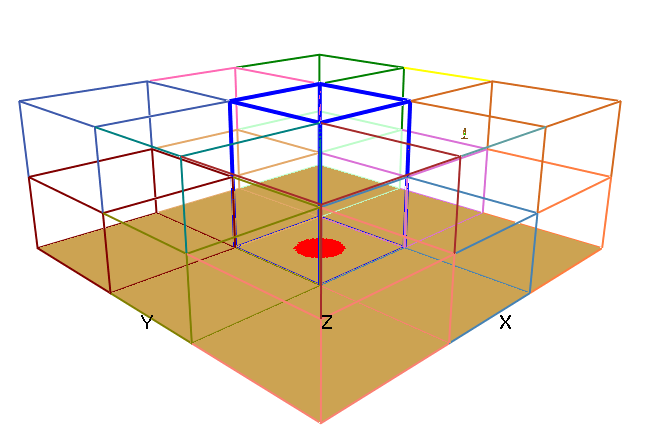
\includegraphics[width=0.83\textwidth]{images/3mRaumMesh.png}
    \caption{Mesheinteilung bei Modell mit 3 m Raumhöhe}
    \label{fig:3mRaumMesh}
\end{figure}

\subsubsection{Modell mit 6 m Raumhöhe}
Das Modell mit 6~m (Abb.~\ref{fig:6mRaumMesh}) hat eine ähnliche Mesheinteilung wie das Modell mit 3~m. 18 Mesh unterteilen den Raum, wobei in diesem Fall zwei Mesh den Bereich über dem Brandherd aufteilen. Das Untere türkis gefärbte ist allerdings auf eine Höhe von 0~m bis 4,5~m Höhe gesetzt, um Flammen im fortgeschrittenen Brandverlauf nicht zu irritieren. Der restliche Raum bis zur Decke wird von einem zweiten Mesh (blau gefärbt) abgedeckt.
\begin{figure}
    \centering
    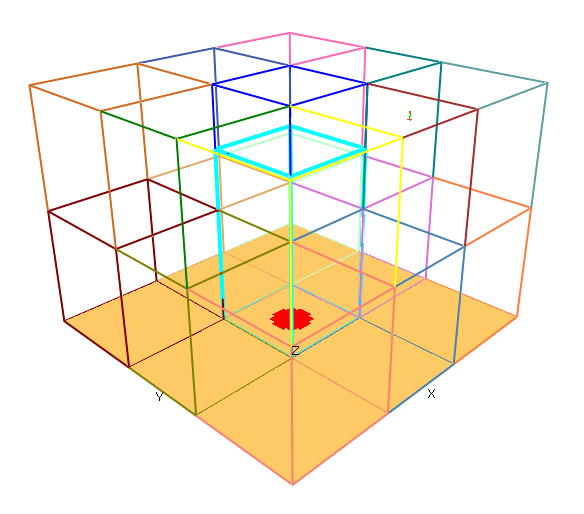
\includegraphics[width=0.83\textwidth]{images/6mRaumMesh.png}
    \caption{Mesheinteilung bei Modell mit 6 m Raumhöhe}
    \label{fig:6mRaumMesh}
\end{figure}
\subsubsection{Modell mit 8 m Raumhöhe}
Das Modell für eine Raumhöhe von 8~m besitzt ähnlich wie das vorherige Modell 18~Mesh mit zwei davon über dem Brandherd. Hier reicht das Untere (türkis gefärbt) von 0~m bis 4,5~m und das Obere (blau gefärbt) von 4,5~m bis 6~m.
\begin{figure}
    \centering
    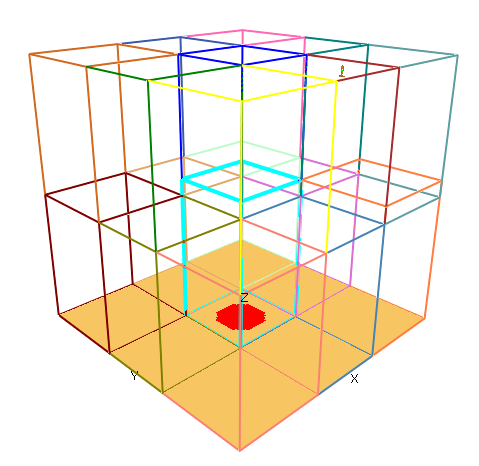
\includegraphics[width=0.83\textwidth]{images/8mRaumMesh.png}
    \caption{Mesheinteilung bei Modell mit 8 m Raumhöhe}
    \label{fig:8mRaumMesh}
\end{figure}

\FloatBarrier


\subsection{Brandherd Definition}
\label{sec:Brandherd}

In den nachfolgenden Zeilen Programmtext wird der Brandherd der Simulation erzeugt. 

\begin{GenericCode}[numbers=none]
&RADI RADIATION=.FALSE. /

&REAC FUEL = 'METHANE', SOOT_YIELD = 0.2, CO_YIELD = 0.1 RADIATIVE_FRACTION=0.2 /

&SURF ID='BURNER', HRRPUA=5500., TAU_MF=0.01 /
&VENT XB=4.5,5.5,4.5,5.5,0.00,0.00, XYZ=5.0,5.0,0.00, RADIUS=0.5, SPREAD_RATE=0.001666, COLOR='RED', SURF_ID='BURNER' /
\end{GenericCode}
In der \code{\&RADI} Zeile wird die Wärmestrahlung für die Simulation deaktiviert. Strahlung hat keinen Einfluss auf die Sprinkleraktivierungszeit in FDS, wirkt sich jedoch, falls aktiviert, negativ auf die Rechendauer der Simulation aus.

Die Zeile \code{\&REAC} definiert zuerst den Brennstoff Methan und anschließend den Rauch- und CO-Anteil aus der Verbrennung. Der Rauchanteil ist nur für visuelle Zwecke vonnöten. Zuletzt wird der Strahlungsanteil auf 0,3 festgesetzt. Da die Wärme eines Feuers in FDS ausschließlich über Konvektion und Strahlung freigesetzt wird, beträgt der Konvektionsanteil somit 0,7 (wie in VDI 6019 -1 \cite[S. 27]{VDI6019B1} definiert). Welcher Brennstoff verwendet wird, hat hier keine Bedeutung mehr, da der Strahlungsanteil und Rauchanteil manuell definiert werden.

Parameter für die Größe, Position und den Verlauf des Brandes werden in die Zeilen \code{\&SURF} und \code{\&VENT} geschrieben. Um eine quadratische Zunahme der Wärmefreisetzungsrate (Heat Release Rate [HRR]) und der Brandfläche zu realisieren, wird eine konstante radiale Ausbreitung der Brandfläche eingestellt. Der \code{TAU\_MF}-Parameter beschreibt die benötigte Zeit in s bis die bei der radialen Ausbreitung neu zugeschalteten Zellen ihre gesamte Wärme freisetzen.
Nachfolgend ist der Rechenvorgang für die Bestimmung der Kenngrößen des Brandherdes skizziert. Zuerst wird die maximale Wärmefreisetzungsrate $\Dot{Q}_{max}$ mit dem Brandintensitätskoeffizienten $\alpha$ und der Zeit $t_{\text{max}}$, bei der die maximale Brandfläche erreicht ist, bestimmt:
\begin{align}
    \Dot{Q}_{max}&=\alpha \cdot t^2_{\text{max}}. \\[20pt]
    \intertext{Die Simulation wird nach 300~s beendet. Somit ist:} \nonumber\\
    \dot{Q}_{max}&= 0{,}047~\text{kW/s²} \cdot (300~\text{s})^2 = 4240~\text{kW}, \\[20pt]
    \intertext{anschließend wird die Kreisfläche des Brandherdes mit r $=0{,}5$ m berechnet:} \nonumber\\
    A&=\pi \cdot r^2 \\[20pt]
    A&= \pi \cdot (0{,}5~\text{m})^2 = 0{,}785~\text{m²} \\[20pt]
    \intertext{und die spez. Wärmefreisetzungsrate (Heat Release Rate Per Unit Area [HRRPUA]  bestimmt:} \nonumber\\
    \dot{q}_{max}&= \frac{\Dot{Q}_{max}}{A}, \\[20pt]
    \dot{q}_{max}&= \frac{4230~\text{kW}}{0{,}785~\text{m²}} = 5385{,}8~\text{kW/s²}.\\[20pt]
    \intertext{Zuletzt wird die Brandausbreitungsgeschwindigkeit kalkuliert:} \nonumber\\
    v &= \frac{r}{t_{\text{max}}},\\[20pt]
    v &= \frac{0{,}5~\text{m}}{300~\text{s}}=0{,}001666~\text{m/s}.
\end{align}

Dies bedeutet, dass am Ende der Simulation der äußere Kreisumfang erreicht wird und 5385,8 kW/m² an Wärme freigesetzt werden. Hier ist anzumerken, dass 5385,8 kW/m² die in der VDI Richtlinie vorgegebenen maximalen spezifischen Wärmefreisetzungsraten (siehe \cite[S.12]{VDI6019B1}) stark überschreitet. 
Dies wird in Kapitel \ref{sec:maxWaermefreisetzungsrate} diskutiert. 

Abb. \ref{fig:HRR} zeigt die fluktuierende Wärmefreisetzungsrate der Simulation im Vergleich zur idealen Wärmefreisetzungsrate auf. Vor allem in den ersten 100~s kommt es zu einer starken Treppenbildung. Dies ist darauf zurückzuführen, dass die 5~cm langen Zellen des Brandherdes nur nach und nach zugeschaltet werden. Allerdings ist auch eine sehr starke Übereinstimmung zwischen der Berechnung und der polynomischen Trendlinie der Simulation zu erkennen.



\begin{figure}[b]
    \centering
    \includegraphics[width=.83\textwidth]{images/HRRKurve.pdf}
    \caption{Vergleich Wärmefreisetzungsrate der Simulation mit Berechnung}
    \label{fig:HRR}
\end{figure}

\subsection{Sprinkler Modell}
\label{sec:SprinklerModell}

Der nachfolgende Auszug aus der Inputdatei positioniert unter anderem den Sprinklerkopf und definiert die Sprinklerkennwerte.
\begin{GenericCode}[numbers=none]
&SPEC ID='WATER VAPOR' /
&PART ID='my droplets', DIAMETER=1000., SPEC_ID='WATER VAPOR' /
&PROP ID='K-11', QUANTITY='SPRINKLER LINK TEMPERATURE', RTI=50., C_FACTOR=0.7, ACTIVATION_TEMPERATURE=68., PART_ID='my droplets', FLOW_RATE=100.0, PARTICLE_VELOCITY=10., SMOKEVIEW_ID='sprinkler_pendent' /
&DEVC ID='Spr-1', XYZ=5.0,1.75,2.97, PROP_ID='K-11' /
\end{GenericCode}
In der \code{\&SPEC}- und \code{\&PART}-Linie werden die Eigenschaften der Wasserpartikel festgelegt, die nach der Sprinkleraktivierung austreten. In dieser Simulation dienen sie allerdings nur zur visuellen Darstellung, da die Unterdrückung des Brandherdes nicht berücksichtigt wird. 
Die \code{\&PROP} Zeile beinhaltet den RTI, C-Faktor und die Auslösetemperatur des Sprinklers.  Außerdem werden die Geschwindigkeit und der Volumenstrom des Sprinklerwassers definiert. Schlussendlich wird die Darstellung des hängenden Sprinklers in Smokeview beschrieben.
Die Zeile \code{\&DEVC} positioniert den Sprinklerkopf im Simulationsraum.

\subsection{Allgemeine Inputparameter}
\label{sec:Allgemeine}

\subsubsection{\&HEAD und \&TAIL}
Zwischen den Zeilen \code{\&HEAD} und \code{\&TAIL} muss der gesamte Programmtext geschrieben werden. Die erste Zeile beinhaltet den Namen und den Titel der Simulation.
\begin{GenericCode}[numbers=none]
&HEAD CHID='OffenerRaum', TITLE='H=3m, a=0,047, C=0' /

&TAIL /
\end{GenericCode}


\subsubsection{\&TIME}
Mit der \code{\&TIME} Zeile wird die maximale Simulationsdauer in Sekunden festgelegt. Nach Ablauf dieser Zeit beendet FDS selbstständig die Simulation, falls nicht schon davor ein "`\code{KILL}"'-Befehl ausgelöst wurde. 
\begin{GenericCode}[numbers=none]
&TIME T_END=300. /
\end{GenericCode}

\subsubsection{\&CTRL}

Der nachfolgende Programmcode definiert eine Steuerung, die nach der Aktivierung des Sprinklerkopfes einen 5 s Timer ablaufen lässt und anschließend die Simulation beendet. Somit kann überflüssige Simulations- und Rechenzeit verhindert werden.
\begin{GenericCode}[numbers=none]
&CTRL ID='kill', FUNCTION_TYPE='KILL', INPUT_ID='delay' /
&CTRL ID='delay', FUNCTION_TYPE='TIME_DELAY', INPUT_ID='Spr-1', DELAY=5. /
\end{GenericCode}

\subsubsection{\&MISC}
In der Zeile \code{\&MISC} wird eingestellt, dass mehr Informationen zur Prozesszuweisung der Mesh in der Konsole angezeigt werden. Dies kann die Fehlersuche vereinfachen.
\begin{GenericCode}[numbers=none]
&MISC VERBOSE=.TRUE./
\end{GenericCode}

\subsubsection{\&SLCF}
In diesem Programmabschnitt werden die Temperatur- und Geschwindigkeitsprofile festgelegt. Hier beispielhaft bei 5 m auf der \emph{X-Achse} und bei 2,95 m auf der \emph{Z-Achse}. Dies ist für die visuelle Auswertung nützlich.
\begin{GenericCode}[numbers=none]
&SLCF PBX=5., QUANTITY='TEMPERATURE' /
&SLCF PBZ=2.95, QUANTITY='TEMPERATURE' /
&SLCF PBX=5., QUANTITY='VELOCITY' /
&SLCF PBX=2.95., QUANTITY='VELOCITY' /
\end{GenericCode}

\subsubsection{\&DEVC}
Um zusätzlich zu der Sprinklerkopftemperatur Daten zu der Gasgeschwindigkeit und -tem\-pe\-ra\-tur zu erhalten, werden sogenannte "`Devices"' definiert. Diese werden auf die gleiche Position des Auslöseelements gesetzt.

\begin{GenericCode}[numbers=none]
&DEVC XYZ=5.0,1.75,2.97, QUANTITY='TEMPERATURE', ID='T-1'/
&DEVC XYZ=5.0,1.75,2.97, QUANTITY='VELOCITY', ID='U-1'/
\end{GenericCode}

\subsubsection{\&DUMP}
Die \code{\&DUMP} Zeile legt fest, in welchem Abstand Daten in den entsprechenden Dateien gespeichert werden (in diesem Fall jede Sekunde).

\begin{GenericCode}[numbers=none]
&DUMP DT_HRR=1.0, DT_DEVC=1.0 /
\end{GenericCode}

\section{Mesh Sensitivity Study}
\label{sec:MeshSS}

Die Auflösung der Simulation ist entscheidend für die Qualität der Ergebnisse. Sie ist allerdings stark situationsabhängig. Während eine Auflösung von 10 cm adäquat für eine größere Entrauchungsstudie in einem Gebäude wäre, wäre dies wahrscheinlich nicht ausreichend bei der Betrachtung eines kleinen Schwelbrandes \cite[S. 44]{FDSUser}. 
Um die für diese Simulationen am besten geeigneten Auflösungen zu ermitteln, wird eine sogenannte Mesh Sensitivity Study (MSS) angestellt. Dieser Begriff beschreibt den Vorgang, die Simulation zuerst mit einer geringen Auflösung zu erstellen und dann schrittweise die Zellenanzahl zu erhöhen bis sich keine merkbaren Unterschiede mehr in den Ergebnissen feststellen lassen. Das zu betrachtende Ergebnis ist in diesem Fall die Sprinklerelementtemperatur. 
Da in dieser Arbeit auch mit verschiedenen Raumhöhen Simulationen angestellt werden, bedarf es mehrerer MSS.

\subsection{MSS für 3~m Raumhöhe}

Für die MSS wurde die Sprinklerelementtemperatur über 300~s untersucht (siehe Abb.~\ref{fig:MSS}). 
\begin{figure}[b]
    \centering
    \includegraphics[width=.75\textwidth]{images/GSS_H=3m.pdf}
    \caption{MSS für eine Raumhöhe von 3~m über einen Zeitraum von 300~s.}
    \label{fig:MSS}
\end{figure}
\begin{figure}
    \centering
    \includegraphics[width=.75\textwidth]{images/GSS_H=3mklein.pdf}
    \caption{MSS für eine Raumhöhe von 3~m über einen Zeitraum von 125~s.}
    \label{fig:MSSklein}
\end{figure}
Vier verschieden hohe Auflösungen werden untersucht, wobei die Simulation mit 2,5~cm Kantenlänge nur für 129~s Simulationszeit bis zum Erreichen von 68~°C Sprinklerelementtemperatur gerechnet wurde. Die Rechendauer betrug zu diesem Zeitpunkt schon fast sechs Tage und es wurde beschlossen, die Simulation vorzeitig zu beenden. Es ist davon auszugehen, dass eine Zellenlänge von 2,5~cm die besten Ergebnisse liefert. In Abb.~\ref{fig:MSSklein} ist zu erkennen, dass in den ersten 130~s zwischen 2,5~cm und 5~cm Zellenlänge die maximale Abweichung ca. 4~s beträgt, während die Abweichung zu Zellenlängen 5~cm und 20~cm erheblich ist mit 15~s bei 38~°C Sprinklerelementtemperatur. Die großen Abweichungen lassen sich damit erklären, dass bei größerer Zellkantenlänge das Zuschalten der ersten Zellen der Brandquelle später passiert als bei einer höheren Auflösung. Aufgrund der zu hohen Rechendauer der Simulationen mit 2,5~cm Zellenlänge wird die nächst bessere Zellenlänge von 5~cm für alle Simulationen mit 3~m Raumhöhe gewählt. 


\subsection{MSS für 6~m Raumhöhe}

Da die Rechenzeit für die Simulation bei einer Raumhöhe von 6~m und 8~m bei einer Kantenlänge von 5~cm sehr hoch ist, soll untersucht werden, ob auch eine Kantenlänge von 10 cm \bzw 20 cm zu rechtfertigen sei. Eine Auflösung von 2,5~cm wird aufgrund der hohen Rechendauer nicht in Betracht gezogen.
Abb. \ref{fig:GSS_H=6m} zeigt zwischen den beiden höher aufgelösten Simulationen meist nur eine geringe Abweichung der Sprinklerelementtemperatur. Die größte Differenz tritt bei 275~s mit 11,4~K auf. Es wird beschlossen, dass eine Zellkantenlänge von 10~cm für Simulationen mit 6~m Raumhöhe geeignet ist. Es wird weiterhin davon ausgegangen, dass auch für eine Raumhöhe von 8~m 10~cm Kantenlänge ausreichend ist.

\begin{figure}
    \centering
    \includegraphics[width=0.75\textwidth]{images/GSS_H=6m.pdf}
    \caption{MSS für eine Raumhöhe von 6~m über einen Zeitraum von 300~s.}
    \label{fig:GSS_H=6m}
\end{figure}

\begin{comment}
\begin{figure}
    \centering
    \resizebox{.8\linewidth}{!}{\includegraphics{images/Rechenzeit.pdf}}
    \caption{Rechenzeit bei verschiedener Mesh-Auflösung}
    \label{fig:Rechenzeit}
\end{figure}



\subsubsection{Rechnerische Untersuchung}

...
\begin{equation}
D^{*}=\left(\frac{\dot{Q}}{\rho_{\infty} \cdot c_{p} \cdot T_{\infty} \cdot \sqrt{g}}\right)^{2/5}
\label{eq:MeshRes}
\end{equation}
\begin{equation}
D^{*}=\left(\frac{0{,}047 \frac{kW}{s^2} \cdot (100s)^2}{1,2\frac{kg}{m^3} \cdot 1{,}005 \frac{kJ}{kg\cdot K} \cdot 293{,}15 \cdot \sqrt{9,8\frac{m}{s^2}}}\right)^{2/5}
\label{eq:MeshRes1}
\end{equation}
...
\end{comment}

\section{Vorangegangene Überlegungen}
\label{sec:vorangegangeneSimulationen}
In diesem Kapitel wird auf die vielen verworfenen Simulationen eingegangen, die im Zuge dieser Arbeit angestellt wurden. Sie dienen vor allem nachfolgenden Arbeiten, die sich mit der gleichen Materie beschäftigen und ihnen Mühen und Aufwand zu ersparen.

\subsection{Modell mit Luftstrahl}
Da der Hauptfokus beim Simulieren der Brandquelle auf dem Abbilden einer $\alpha \cdot t^2$ -Kurve bestand, wird versucht, die Brandquelle mit einem Heißluftstrahl zu ersetzen. Hierfür wird ein Luftdurchlass am Boden des Raumes definiert, der Luft bei konstantem Volumenstrom in den Raum befördert. Die eingeblasene Lufttemperatur folgt einer vorgegebenen quadratischen Kurve bis die maximale Temperatur am Ende der Simulationsdauer erreicht ist. Die maximale Temperatur kann mithilfe der Formel $\Dot{Q}=\dot{m}\cdot c_p \cdot \Delta \vartheta$ berechnet werden. Für die visuelle Veranschaulichung werden dem Luftstrahl Rauchpartikel zugegeben. Der zeitliche Verlauf ist in Abb. \ref{fig:Luftstrahl} zu erkennen. Bei 2,1~s erreicht der Strahl die Decke und breitet sich anschließend an der Decke aus. 
Der Strahl aus dem Boden ist sehr geradlinig und besitzt nicht die charakteristischen Merkmale eines richtigen Feuers. Außerdem weist er keine Wirbel auf und die Temperatur und Geschwindigkeit sind uniform über den gesamten Querschnitt des Strahls. Während diese Methode bei näherer Betrachtung möglicherweise eine Alternative zur Simulation eines echten Feuers sein könnte, wird sie in dieser Arbeit aufgrund der Unsicherheiten nicht weiter fortgeführt.

\begin{figure}%
\centering
\subfigure[][]{%
\label{fig:Luftstrahl1}%
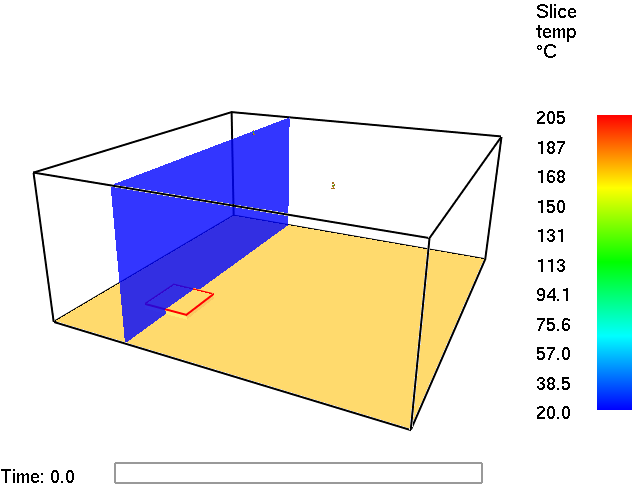
\includegraphics[width=.45\textwidth]{images/FDSBilder/Luftstrom1.png}}%
\hspace{8pt}%
\subfigure[][]{%
\label{fig:Luftstrahl2}%
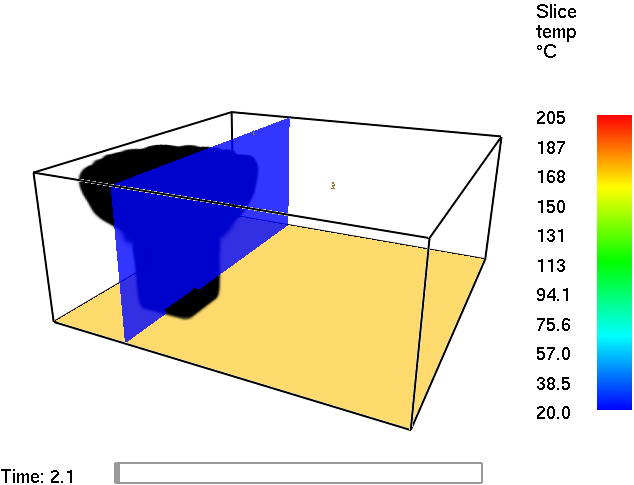
\includegraphics[width=.45\textwidth]{images/FDSBilder/Luftstrom2.png}}\\
\subfigure[][]{%
\label{fig:Luftstrahl3}%
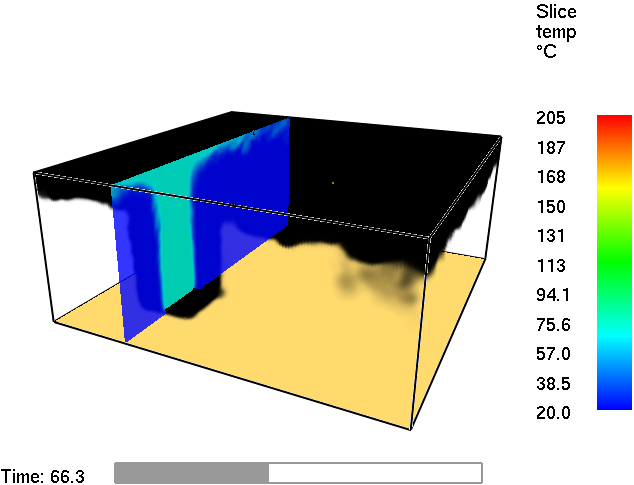
\includegraphics[width=.45\textwidth]{images/FDSBilder/Luftstrom3.png}}%
\hspace{8pt}%
\subfigure[][]{%
\label{fig:Luftstrahl4}%
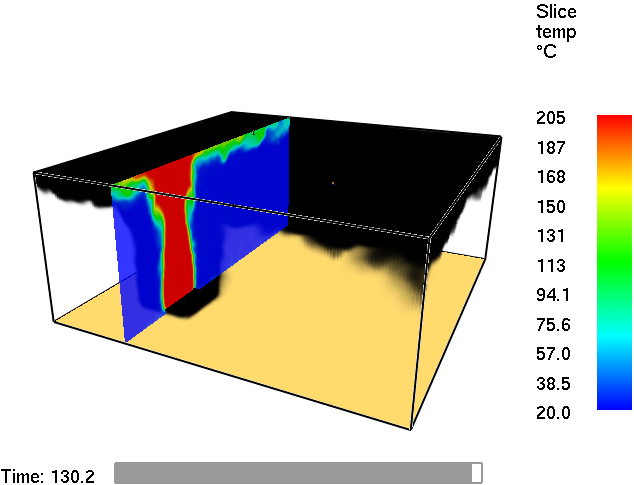
\includegraphics[width=.45\textwidth]{images/FDSBilder/Luftstrom4.png}}%
\caption[A set of four subfigures.]{Zeitlicher Verlauf der Simulation mit Luftstrahl und Temperaturprofil in Smokeview.}%
\label{fig:Luftstrahl}%
\end{figure}

\begin{comment}
\begin{GenericCode}[numbers=none]
&TIME T_END=300 /
&SURF ID='Blower', VEL=-6.0, TMP_FRONT=1057.0, RAMP_T='ramp', SPEC_ID(1)='SMOKE SPECIES', MASS_FRACTION(1)=1 /
&VENT XB=1.25,2.25,1.25,2.25,0.1,0.1, COLOR='RED', OUTLINE=.TRUE., SURF_ID='Blower' /
&RAMP ID='ramp', T=0, F=0 /
&RAMP ID='ramp', T=30, F=0.01 /
&RAMP ID='ramp', T=60, F=0.04 /
&RAMP ID='ramp', T=90, F=0.09 /
&RAMP ID='ramp', T=120, F=0.16 /
&RAMP ID='ramp', T=150, F=0.25 /
&RAMP ID='ramp', T=180, F=0.36 /
&RAMP ID='ramp', T=210, F=0.49 /
&RAMP ID='ramp', T=240, F=0.64 /
&RAMP ID='ramp', T=270, F=0.81 /
&RAMP ID='ramp', T=300, F=1.0 /
\end{GenericCode}
\end{comment}
%%


\subsection{Modell mit "`Säule"'}
Einen Versuch, die Rechenzeit bei gleichbleibenden Ergebnissen zu verringern, wird bei dem Modell mit "`Säule"' unternommen. Es wird davon ausgegangen, Bereiche, die nicht essentiell für die Simulation sind, niedriger aufzulösen als Bereiche mit kritischen Vorgängen wie \zB beim Brandherd oder Sprinklerkopf. 
Aufgrund dieser Aussage wird der Versuch angestellt, einen mit 5~cm hochaufgelösten Bereich von der Brandquelle bis zum Sprinklerkopf zu modellieren. So soll garantiert werden, dass kein Informationsverlust von der Brandquelle bis zum Sprinklerkopf auftritt. In Abb.~\ref{fig:Grundriss} ist der Grundriss für den Simulationsraum (Höhe gleich 3 Meter) zu sehen. Der dazugehörige Schnitt ist in Abb.~\ref{fig:Schnitt} dargestellt. 
\begin{figure}
    \centering
    \includegraphics[width=0.8\textwidth]{images/Grundriss.pdf}
    \caption{Grundriss der Simulation}
    \label{fig:Grundriss}
\end{figure}
\begin{figure}
    \centering
    \includegraphics[width=0.8\textwidth]{images/Schnitt.pdf}
    \caption{Schnitt A-A der Simulation}
    \label{fig:Schnitt}
\end{figure}
Die Mesh 1, 2, 3, 4, 11 und 12 werden mit einer Zellenkantenlänge von 10~cm aufgelöst, während die Mesh 5, 6, 7, 8, 9 und 10 mit einer Kantenlänge von 5~cm aufgelöst werden. Obwohl die Rechenzeit mithilfe dieser Methode deutlich gesenkt werden kann, kam es doch zu einer erheblichen Abweichung zu der Referenzsimulation aus der Mesh Sensitivity Study wie aus Abb. \ref{fig:GSS_mit_Saeule} ersichtlich wird. Bis zu einer Simulationszeit von ungefähr 210~s kommt es zu keinen großen Abweichungen der Sprinklerelementtemperatur. Ab diesem Zeitpunkt variiert die Temperatur jedoch bis zu 40~°C zwischen den beiden Verläufen. Dies ist möglicherweise damit zu erklären, dass der Plume die Breite der hochaufgelösten Säule von 2~m bei 210~s überschreitet und dies an den Meshgrenzen zu Informationsverlust führt. Das Modell wird nicht weiter betrachtet und es wird dazu übergegangen, den gesamten Raum gleich hoch aufzulösen.
\begin{figure}
    \centering
    \includegraphics[width=.83\textwidth]{images/GSS_mit_Saeule.pdf}
    \caption{Vergleich der Sprinklerauslösezeit}
    \label{fig:GSS_mit_Saeule}
\end{figure}

\subsection{Modell mit 20 Mesh}
Nachdem das Modell mit "`Säule"' als unzureichend eingeordnet wird, wird versucht das 3~m Modell mit den gesamten für die Arbeit zur Verfügung stehenden Rechenkernen bzw. Mesh aufzulösen. Hierfür wird wie im endgültigen Modell ein "`Tic-Tac-Toe"' Feld als Grundlage gewählt. Statt wie in Kap.~\ref{sec:modellmit3mraumhöhe} zu sehen ist, werden in diesem Modell jedoch vier Mesh über dem Brandherd angeordnet. Diese Mesh durchteilen die Flammen und es kommt zu Informationsverlust an den Meshgrenzen. Das Modell wird nicht weiter betrachtet.












